\ylDisplay{Kujutis} % Ülesande nimi
{EFO žürii} % Autor
{piirkonnavoor} % Voor
{2018} % Aasta
{P 10} % Ülesande nr.
{3} % Raskustase
{
% Teema: Valgusõpetus
\ifStatement
Joonisel on kujutatud läätse keskpunkt $O$, fookus $F$ ning kujutis $A'B'$ . Konstrueerige kujutise tekitanud ese.
\begin{center}
	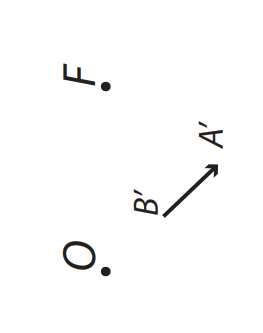
\includegraphics[width=0.5\linewidth]{2018-v2p-10-yl.PNG}
\end{center}
\fi
\ifHint
Esmalt tuleb joonistada optiline peatelg ja lääts. Sellest tuleb mõista, et tegemist on näiva kujutise ning nõgusläätsega. Ainult nõguslääts saab tekitada kujutise läätse ja fookuse vahele.
\fi
\ifSolution
Joonistame optilise peatelje. Joonistame läätse (lääts risti optilise peateljega). Tuleb mõista, et tegemist on näiva kujutise ning nõgusläätsega. Ainult nõguslääts saab tekitada kujutise läätse ja fookuse vahele. Joonistame kujutise otstest $A'$ ja $B'$ kiire läbi läätse keskpunkti $O$. Tuleb mõista, et ese asub sirgel, mis läbib punkte $A'$ , $B'$ , $O$. Joonistame punktist $A'$ kiire läbi fookuse $F$, mis lõikab läätse punktis $D$. Joonistame punktist $D$ optilise peateljega paralleelse kiire, mille lõikepunkt läätse keskpunkti läbiva kiirega ongi eseme ots $A$. Joonistame punktist $B'$ kiire läbi fookuse $F$, mis lõikab läätse punktis $C$. Viimaks joonistame punktist $C$ optilise peateljega paralleelse kiire, mille lõikepunkt läätse keskpunkti läbiva kiirega ongi eseme ots $B$.
\begin{center}
	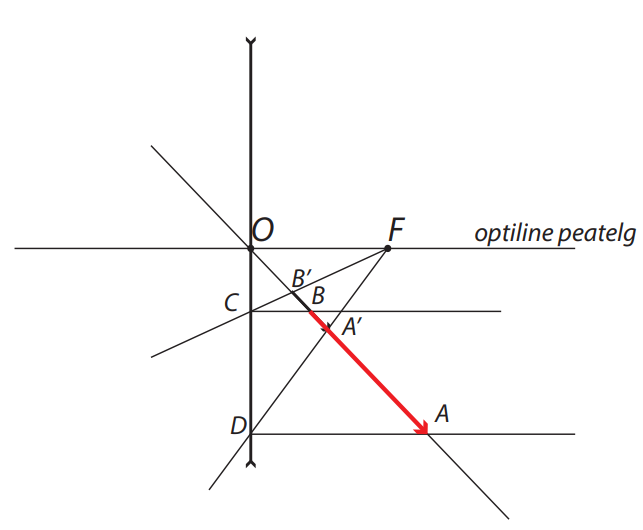
\includegraphics[width=0.5\linewidth]{2018-v2p-10-lah.PNG}
\end{center}
\fi
}
